\documentclass[letterpaper,twocolumn,11pt]{article}
\usepackage{usenix,epsfig,endnotes,amsmath}
\usepackage{alltt}
\usepackage[margin=1in, paperwidth=8.5in, paperheight=11in]{geometry}
\usepackage{url}

\title{NFS Trace Deconstruction: 
Server Side NFS Identification and Client-Side Packet Tracing in a Virtualized Environment}
\author{Rob Jellinek and Adam Vail}
\begin{document}
\maketitle

\begin{abstract}
This paper investigates server-side methods for determining whether an NFS client is virtualized or native. We perform client-side and server-side network traces that identify two key differences that can be used as heuristics in identifying virtualized clients. First, virtualized clients using bridged networking can often be detected by the first three octets of their MAC address at the link layer, which are set to unique defaults by most common virtualization platforms. Second, virtualized clients using user-mode networking experience substantially reduced bandwidth due to processing overhead in their network stack. Clients can then be distinguished according to bandwidth profiles. Finally, we investigate the sources of the reduced user-mode networking bandwidth and identify the memory management overhead inherent in network address translation as the primary contributor to slowdown.
\end{abstract}

\section{Introduction}
This paper investigates how an NFS server can differentiate native, non-virtualized NFS clients from clients running on virtual machines. 
Ultimately, it is desirable for an NFS server to be able to identify and group all virtual machines resident on the same physical machine. Such identification and grouping would allow the server to coalesce its outgoing network traffic to the virtual machines, in essence performing VM-based redundancy elimination. This would lead to better NFS performance, and lower network utilization.

Our approach consisted of three parts. First, we searched through the NFS 4.0 RFC specification \cite{shepler2003network} to find operations that could potentially differ between the virtualized and native context, or otherwise uniquely mark the origin of the client machine. Second, we performed a number of client and server-side network traces on NFS 4.0 \texttt{mount} operations as well as file transfers with the goal of isolating differences in the action of the NFS protocol in the virtual and native settings. Finally, we timed NFS reads of varying sizes in the virtual and native settings in order to determine if timing differences could be used to distinguish native from virtual clients. 

We learned several things from these investigations. First, we were unable to differentiate any aspect of the NFS protocol in the virtual setting from its behavior in the native setting at the application layer, either in our reading of the NFS 4.0 RFC or in our network traces. This is not surprising, as there is nothing that should inherently differ about the behavior of the application layer in a virtual machine. Thus, unless explicit signals are incorporated into the NFS protocol for the purpose of identifying a client as virtualized, nothing from the vanilla NFS protocol implementation seems to identify the platform of the client. 

However, we were able to establish two heuristics for identifying virtualized NFS clients. First, our network traces showed that although NFS application-layer semantics were indistinguishable, VM-based clients could be identified by a unique MAC address assigned by default to virtual NICs when the VM is using bridged networking. Second, our NFS read timings showed that virtualized clients using user-mode (NAT) networking experience a substantial drop in bandwidth compared to a native-client baseline. By profiling client accesses and establishing a baseline bandwidth, it is possible to use bandwidth profiles to identify a virtualized guest in a controlled environment.

The remainder of our work focused on determining why and how user-mode networking suffers such a dramatic slowdown compared to bridged networking. In particular, we trace and identify the key points in the code path of KVM+QEMU user-mode networking that cause this slowdown.

The rest of the paper is organized as follows. Section \ref{sec:NFS} describes our network trace collection and timing tests, and the corresponding heuristics for differentiating native and virtualized NFS clients. Subsection \ref{subsec:networkIntro} introduces and compare user-mode and bridged networking, which form the basis of our heuristics for differentiating clients by MAC address (Subsection \ref{subsec:macaddrs}) and bandwidth profiles (Subsection \ref{subsec:BWprofiles}). Finally, in Section \ref{sec:trace} we examine the source of slowdown in user-mode networking in KVM+QEMU.


%******************************
%[TODO: incorporate below]
%
%Looking lower in the network stack, however, we found that the MAC addresses assigned to the virtual NICs of bridged connections took on default values under all the virtualization platforms we investigated, which would allow a server to distinguish the virtualization platform of VM-based client applications in these cases. We discuss our findings and the implications in more detail in Subsection \ref{subsec:macaddrs} below. Finally, we found that NFS reads from a KVM+QEMU VM using NAT networking and virtio PCI paravirtualized network driver took an average of 72\% longer than reads from a native-hardware client, while NFS reads from a KVM+QEMU VM using bridged networking with the virtio driver took an average of 26\% longer than the client running on the same underlying native-hardware setup. Our data collection and analyses are discussed below in Section \ref{sec:NFSTiming}. 
%******************************

%TODO: change section title
\section{Differentiating Native and Virtualized NFS Clients}
\label{sec:NFS}

\subsection{Experimental Setup}
\label{subsec:expSetup}
The traces and timing experiments discussed below were run on a simple two-node topology connected by a Cisco E-2000 gigabit router. The client was a Thinkpad T60 with a dual-core 1.83GHz Intel T2400 CPU, 2GB RAM, and an Intel 82573L gigabit NIC. The server was an AMD Opteron 148 operating at 1GHz, with 1GB of RAM and a gigabit on-motherboard NIC. The client and server both used ext4 as their primary filesystem, and the client KVM+QEMU guest VM used ext4 on an 8GB QCOW2 virtual disk. The client was running Ubuntu 12.04LTS natively and in its guest VMs, and the server was running CentOS 5.2.

The network traces we collected were executed with the flags \texttt{tcpdump -vvnnXSs 1536} in order to examine the full contents of each NFS packet exchanged between the client and server.

\subsection{User-mode/Bridged Networking}
\label{subsec:networkIntro}
Both of the heuristics we discuss below rely on key differences in network behavior and timing caused by the two main virtual networking configurations used by guest VMs. Guest VMs can be configured to run either user-mode, or bridged networking.

User-mode networking performs network address translation (NAT) behind the host, which isolates guest VMs from the outside network. That is, no entities outside the physical host's network can see the guest VMs, and so without incorporating port-forwarding from the host, those guests cannot be contacted from the outside. Importantly, this also has the effect that all guest VMs share a common IP and MAC address with the host; when the guest has an established TCP session open and the host receives packets destined for that guest, the host demultiplexes those packets and forwards them to the correct guest. 

KVM+QEMU uses the SLiRP protocol \cite{slirp} to perform network address translation. SLiRP was originally used to emulate TCP/IP and provide transport-layer functionality for users with dial-up connections. The emulation code has been incorporated into the main branch of KVM+QEMU, and has been adapted to provide support for user-mode networking.

Bridged networking, on the other hand, uses a TAP device that is configured on the host. Both the physical NIC and the TAP device must be connected to a virtual network bridge on the host. Creating the TAP device requires root access, and so is not an option for all users. Guest VMs attach to the TAP device through their virtual interfaces and participate as fully fledged members of the network. This means that their virtual NICs are assigned unique IP addresses that are visible to the outside network, as well as MAC addresses that must be unique within the network.

\subsection{Identifying Bridged Hosts by MAC Address}
\label{subsec:macaddrs}
Since under virtual bridged networking the guest is assigned its own IP and MAC address and appears as a separate host on the network, it must get its IP and MAC address from some source. Typically, it is assigned its IP via DHCP or static assignment in a similar manner to the physical host. But its MAC address must first be assigned by some other means. Here, we can take advantage of the behavior of most virtualization platforms, which assign a default MAC address to the guest's virtual NIC unless a particular MAC address is otherwise specified. The first three octets of each default hypervisor-assigned 48-bit MAC address are fixed according to the virtualization platform, which allows us to use the MAC address to identify the client's underlying platform. This MAC address is visible to the server in the MAC address fields of the Ethernet headers exchanged with the client. See Table \ref{tab:macaddrs} for a list of default MAC addresses assigned to virtual NICs under common virtualization platforms. 

This helps us distinguish virtual from native clients to some extent, but still leaves a lot to be desired if we wish to identify and \emph{group} VM-based NFS clients. First, in the bridged context, it is possible for a client VM user to specify their MAC address to be anything they desire. These defaults are merely that: default settings allocated by the virtualization manager or hypervisor if the VM user or administrator does not specify an alternative address. So there is certainly a chance for false negatives, where virtual machines using bridged networking on a certain platform cannot be identified by their MAC address because the default MAC address is not used. Second, the identification is overly broad: the NFS server can detect that it is talking with a KVM+QEMU or VMWare guest VM, for example, but it is not possible to determine that the guest VM resides on a given physical machine based on this information alone. Finally, this approach works only for guests using bridged networking, since NATed guests use the IP and MAC address of their underlying physical host.

\begin{table*}[htb]
		\centering
		\begin{tabular}{|l|l|}
		\hline
			Virtualization Platform & MAC \\
		\hline
		\hline
			KVM+QEMU & 52:54:00 \\
			VMware ESX 3, Server, Workstation, Player	& 00-50-56, 00-0C-29, 00-05-69 \\
			Microsoft Hyper-V, Virtual Server, Virtual PC	& 00-03-FF \\
			Parallells Desktop, Workstation, Server, Virtuozzo & 00-1C-42 \\
			Virtual Iron 4 & 00-0F-4B \\
			Red Hat Xen	& 00-16-3E \\
			Oracle VM	& 00-16-3E \\
			XenSource	& 00-16-3E \\
			Novell Xen & 00-16-3E \\
			Sun xVM VirtualBox & 08-00-27 \\
		\hline
		\end{tabular}
	\caption{First three octets of default MAC addresses by virtualization platform \emph{(Source:http://www.techrepublic.com/blog/networking/mac-address-scorecard-for-common-virtual-machine-platforms/538)}}
	\label{tab:macaddrs}
\end{table*}


\subsection{Identifying NATed Host by Bandwidth Profiles}
\label{subsec:BWprofiles}	

\begin{figure}[htb]
		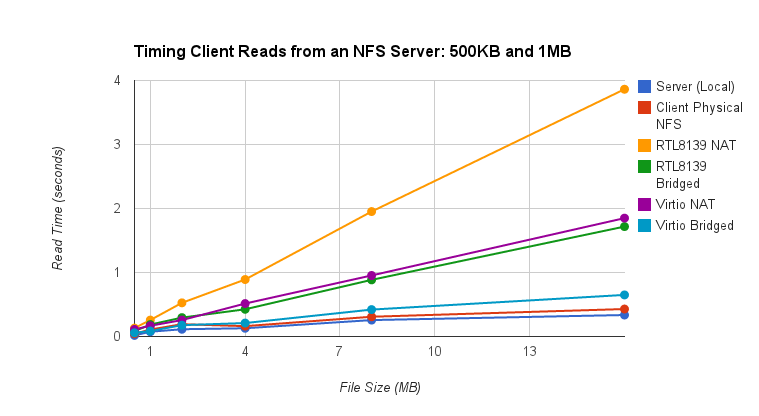
\includegraphics[scale=0.34]{timing_small.png}
	\caption{When reading small files, bandwidth profiles are not yet clearly ordered.}
	\label{fig:timing_small}
\end{figure}

\begin{figure}[htb]
		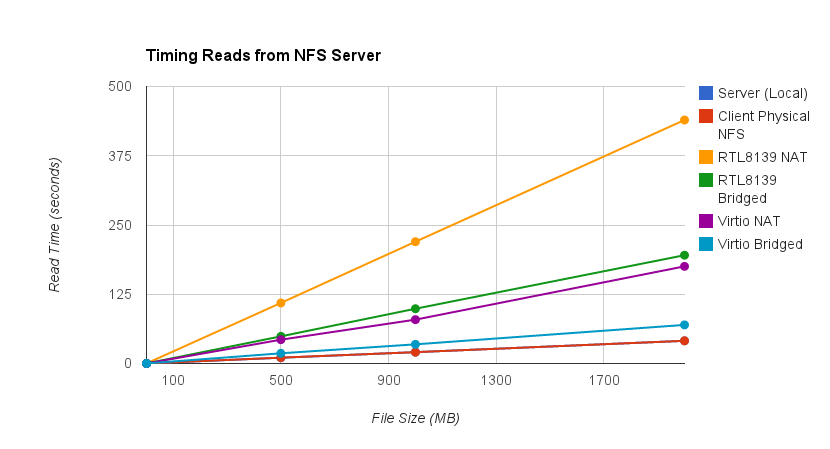
\includegraphics[scale=0.3]{timing_large.png}
	\caption{When reading larger files, the bandwidth profiles are clearly differentiated.}
	\label{fig:timing_large}
\end{figure}

The MAC address distinction does not help us in the case of VM-based clients that are using user-mode (NAT-based) networking instead of bridging, as NATed guests are not visible to the rest of the network and do not have an externally identifiable IP and MAC address. As discussed above, all guest VM traffic is rewritten inside the host to contain the MAC and IP addresses of the host NIC. However, user-mode networking suffers from a substantial slowdown compared to physical or bridged hosts. In a controlled environment, an NFS server can take advantage of this dramtically decreased bandwidth relative to a native-client baseline to conclude that the client is virtualized. 

Figures \ref{fig:timing_small} and \ref{fig:timing_large} show the results of timing tests in which the client VMs under various networking configurations read 500KB, 1MB, 500MB, 1GB, and 2GB files from an NFS server according to the configuration describe in Subsection \ref{subsec:expSetup}. Files were read in 4KB blocks, and file buffer caches were cleared between tests by running \texttt{echo 3 > /proc/sys/vm/drop\_caches}. Figure \ref{fig:timing_small} shows that when reading smaller files, the bandwidths of the various client-VM networking configurations have not yet achieved a stable relative ordering. However, when reading larger files, as shown in Figure \ref{fig:timing_large}, a clear relative bandwidth ordering emerges.

Not surprisingly, reads on the server itself (directly from the local ext4 file system) were fastest and were mirrored almost exactly by reads from the NFS client running on native hardware. Note that the reads performed locally on the server and from the native client differed by only 43 milliseconds across all tests, so their lines are coincident in Figure \ref{fig:timing_large}. Of the virtualized clients, using the paravirtualized virtio driver under bridged networking imposed only a slight overhead relative to the native-client baseline. However, switching to either the fully emulated RealTek RTL8139 virtual network driver or using NATed instead of bridged networking imposed a substantial bandwidth penalty. Doing both (using the RTL8139 under user-mode networking) results in 10.7x slowdown relative to our baseline. 

Table \ref{tab:NFSBandwidthProfiles} shows the bandwidths observed across the different network configurations of our client KVM+QEMU VM when performing the NFS read-timing tests. Importantly, the bandwidths are highly differentiated. In a controlled environment, this would allow an NFS server to take a ``bandwidth fingerprint'' of an NFS client by performing a sustained read and recording the bandwidth, and infer from its bandwidth whether the client was running on a native or virtualized platform. 

\begin{table}[htpb]
		\begin{tabular}{|l|l|}
			\hline
			\textbf{Client Network Stack} & \textbf{Bandwidth} (MB/sec) \\
			\hline
			Native & 48.3 \\
			Virtio Bridged & 28.3 \\
			Virtio NAT & 11.9 \\
			RealTek Bridged & 10.2 \\
			RealTek NAT & 4.6 \\
			\hline
		\end{tabular}
	\caption{NFS Bandwidth Profiles}
	\label{tab:NFSBandwidthProfiles}
\end{table}

\subsection{NFS Client Identification Conclusions}
Given a lack of signals at the application layer that might differentiate native and virtual NFS clients, the two heuristics described above provide an NFS server with a rough means of separating the two classes of clients. When combined, the heuristics should provide a good indication of a client's underlying platform. If the client is using bridged networking under a default configuration, their bandwidth may be close to the native-client baseline but their MAC address will identify them as virtualized with a high degree of certainty. On the other hand, if the client is using user-mode networking, they will not be identifiable based on their MAC address, but their substantially decreased bandwidth can suggest their use of user-mode networking. 

In the next section, we shift gears to try to isolate the origin of the decreased bandwidth of user-mode networking from the client side.

\section{Investigating User-mode Networking}
\label{sec:trace}

The results in Figure \ref{fig:timing_large} led us to investigate why user-mode networking incurs such a large delay over bridged networking.
We traced the control path for packets going from a guest VM out to the network as well as from the network to a guest VM under both networking modes.
We focus on packets going from the guest to the network since this path incurs the largest overhead in the system.
The path from the network to the guest is detailed in the Appendix. 
We chose the RealTek 8139 driver because it is fully emulated by the system (unlike the paravirtualized virtio driver) and thus incurs the largest amount of delay.
The RTL8139 driver is also one of the most widely supported drivers and is the default for user-mode networking when the user does not specify an explicit configuration.
While Figure \ref{fig:timing_large} clearly shows a difference in performance between the drivers, the distinction between the different modes of networking was through the use of SLiRP and not specific to the driver.
%
%We were particularly interested because this is the default network configuration in KVM+QEMU if a user does not specify a configuration explicitly. 
%It is likely the default because the RTL8139 is widely supported, and because users will not be able to use bridged networking if they cannot set up a TAP device on their machine, a process that requires root access. 
%Because of that, it is most likely to be accessible, but as we can see, is also the least performant.
%
%In order to determine where the bottlenecks are occurring using the RTL8139, we traced the code path of a packet from the guest's application layer through the guest network stack and QEMU network emulation code using \texttt{callgrind} and \texttt{gdb}. 
%We discuss the traces and relevant functions in the code path for the guest transmissions below. 
%We provide an outline of the traces involved in the guest's receive path in the Appendix, along with the code path followed by packets on the transmit side that are shared by both the user-mode and bridged code. 

\subsection{Transmission from a Guest to the Network}
\label{subsec:usermode}

The control flow of a packet is split into two parts.
The packet first travels through the networking stack of the guest VM, and then moves through code in QEMU that is shared by both user-mode and bridged networking.
Once QEMU determines which mode of networking is being used, the code paths diverge and the sources of the slowdown become evident.

\subsubsection{Shared Control Path}
\begin{figure*}[!ht]
	\centering
		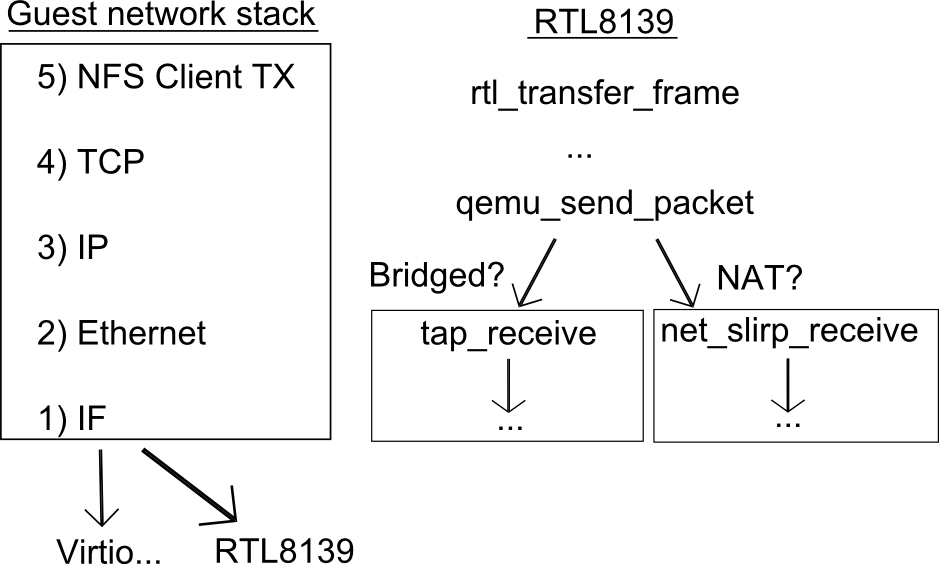
\includegraphics[scale=0.6]{codepath1}
	\caption{Virtualized client TX code path under bridged and user-mode (NAT) networking using the RTL8139 fully emulated driver. Both start at the top of the guest network stack, but diverge after \texttt{qemu\_deliver\_packet}.}
	\label{fig:codepath1}
\end{figure*}

Figure \ref{fig:codepath1} presents the code path originating at a guest VM's application layer.
The packet moves down the guest's networking stack to what it believes to be the physical network interface card.
At this point the packet is passed to whatever driver has been selected by the user.
In KVM+QEMU the options are \texttt{rtl8139}, \texttt{virtio}, or \texttt{e1000}.
Once the packet is processed by the driver, it encounters a sizeable amount of shared code which is designed to determine which mode of networking is being used and passes the packet off to the
correct function.
If the guest is bridged then the packet is passed to \texttt{tap\_receive}, otherwise \texttt{net\_slirp\_receive} is invoked.

\begin{figure*}[!ht]
	\centering
		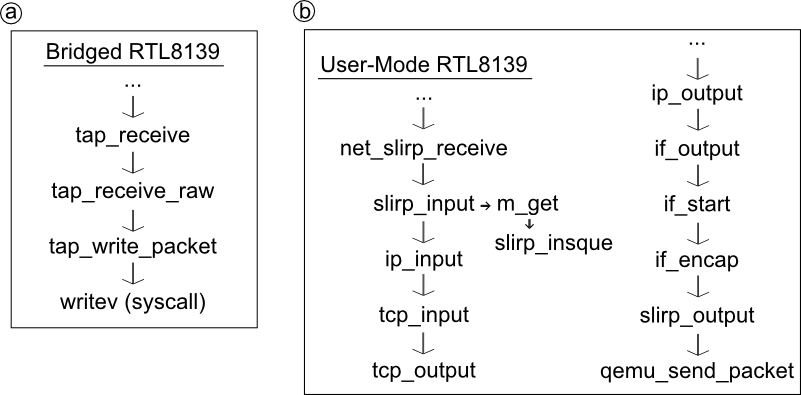
\includegraphics[scale=0.6]{codepath2_alt}
	\caption{Important functions in the divergent branches of bridged and user-mode networking.}
	\label{fig:codepath2}
\end{figure*}
\subsubsection{Bridged Packet Flow}
Figure \ref{fig:codepath2}a depicts the code path for bridged networking.
The code is relatively straight forward and concise.
\texttt{Tap\_receive} simply verifies the TAP state and then calls \texttt{tap\_receive\_raw}.
\texttt{Tap\_receive\_raw} translates the packet into iovectors.
\texttt{Tap\_write\_packet} is just a wrapper around the \texttt{writev} system call, checking the return value and error code.
Finally, \texttt{writev} writes the iovectors to the TAP.

\subsubsection{User-mode Packet Flow}

Figure \ref{fig:codepath2}b shows a flowchart of the user-mode networking path.
QEMU's SLiRP implementation, as you can see, requires considerably more code to process a packet compared to bridged networking.
The control flow starts when the RealTek driver passes the packet to the \texttt{net\_slirp\_receive} function.
\texttt{Net\_slirp\_receive} simply passes the packets along to \texttt{slirp\_input} along with the SLiRP connection state.
\texttt{Slirp\_input} calls two functions before the control flow continues: first to \texttt{m\_get}, which in turn calls \texttt{slirp\_insque}.
In \texttt{m\_get}, memory is allocated and then passed on to \texttt{slirp\_insque} which manages a free list of memory.
%The code attempts to reuse memory efficiently, but even with this optimization, we'll see that it still spends the majority of its time managing memory.
The chunk of memory is then returned to \texttt{slirp\_input} where the packet is then copied into the buffer.

Once the packet has been copied, it is passed ``up the stack'' to \texttt{ip\_input}. 
\texttt{Ip\_input} uses the IP headers to sanity check different aspects of the packet such as the checksum and length.
If for some reason the packet has been fragmented, it also attempts to reassemble it.
If the packet is found to be malformed then it is dropped and its memory is freed.

If the packet passes the tests in \texttt{ip\_input} it moves to \texttt{tcp\_input}.
\texttt{Tcp\_input} is a direct implementation of the TCP specification from September, 1981.
It does all the standard operations associated with TCP such as calculating the receive window and updating the TCP control block that QEMU maintains.
It then strips the guest's IP and TCP headers from the packet, leaving just the TCP payload, which is passed to \texttt{tcp\_output}.
It is at this point that the packet starts to move back ``down the stack'' to be put out onto the wire.
\texttt{Tcp\_output} handles TCP timers to determine when a packet should actually be sent.
Once a packet is cleared to send, the TTL and TOS fields are filled in and the packet is passed along.
With the transport layer complete the packet moves to \texttt{ip\_output} where its IP header fields are filled in with the host's information.
At this point the packet is fully formed.

It is handed off to \texttt{if\_output} which manages two different packet queues, \texttt{fastq} and \texttt{batchq}.
If a packet has the \texttt{IPTOS\_LOWDELAY} flag set, then it is placed on the \texttt{fastq}, which is intended for packets from an interactive application.
Otherwise, latency insensitive packets are placed on the \texttt{batchq}.
Each output queue is a doubly linked list of doubly linked lists of mbufs, each belonging to a separate socket.
This is intended to ensure that packets are fairly chosen for transmission across all the sockets of a system.
If a socket is found that does not have a linked list yet, then another is created.
To create the linked list, \texttt{if\_output} calls \texttt{m\_get} which, again, calls \texttt{slirp\_insque}.
The packet then moves on to \texttt{if\_start} which services both the \texttt{fastq} and the \texttt{batchq}.
As the names would indicate, the \texttt{fastq} is serviced first.
\texttt{If\_start} also cleans up the memory from each packet once the functions under it return.

Once a packet is chosen by \texttt{if\_start} it is passed to \texttt{if\_encap}.
Here the packet is prepared for going out on the wire by copying the packet header information into the appropriate header structs.
Finally, \texttt{slirp\_output} receives the packet which simply gives it to QEMU to be put on the wire through \texttt{qemu\_send\_packet}. 
%At this point qemu takes over and the rest of the control path is no longer dictated by the fact that usermode networking is in use.

\subsection{Code Path Timing}
\label{codePathTiming}
We timed the diverging sections of user-mode and bridged networking transmission paths. 
We began timing both paths at the function \texttt{rtl8139\_transfer\_frame}, ending the user-mode timing at \texttt{slirp\_output} and the bridged timing at \texttt{tap\_write\_packet}. 
The user-mode path took an average of 1.1 milliseconds, while the bridged path took an average of 44 microseconds, demonstrating a factor of 25 slowdown for user-mode networking relative to bridged.

\begin{figure}[htbp]
	\centering
		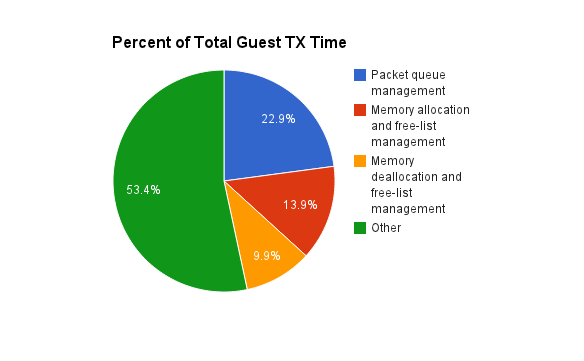
\includegraphics[scale=0.5]{usermodeTXtime}
	\caption{Almost half of the time spent in user-mode networking is spent in memory management.}
	\label{fig:usermodeTXtime}
\end{figure}

We then instrumented the SLiRP functions and found that almost 50\% of the overhead in user-mode networking is due to the memory management that takes place in \texttt{slirp\_input},
\texttt{m\_get}, \texttt{slirp\_insque}, \texttt{if\_output}, \texttt{if\_start}, \texttt{m\_free}, and \texttt{slirp\_remque}.
The most expensive of these functions was the management of the doubly linked lists of doubly linked lists of mbufs done in \texttt{if\_output} and \texttt{if\_start} which accounts for 22.9\%
of the transmit time.
Therefore, the management of memory was seen to be a major contributor to the slow down in user-mode networking.
Bridged networking does not have this problem since there is no need to manipulate the packet, which allows it to use the TAP to place the packet directly on the wire.

We also note that user-mode networking is essentially duplicating much of the work already done by the guest's network stack in order to rewrite the correct header fields to make the packet
look as though it originated from the host machine.
A packet must travel down the guest's networking stack, back up to the transport layer, and then back down before finally getting sent.



%\subsection{RealTek 8139 NAT: Guest Transmit}
%User-mode networking under QEMU uses network address translation (NAT) in order to allow a guest VM to establish connections with outside networks. QEMU performs address translation using a protocol from the 1990s known as SLiRP, which was originally used to provide TCP/IP access to dial-up shell account users by emulating the TCP/IP stack. Though that usage is largely obsolete, the same address translation techniques are applied in QEMU user-mode networking to provide NAT functionality.

\section{Conclusions}
We began searching for methods by which an NFS server could differentiate native from virtualized clients, and arrived at two conclusions. First, bridged clients can be detected by matching the first three octets of their MAC address against a list of default MAC address prefixes used by virtualization platforms for their bridged guest VMs. If a match is found, this indicates the client is virtualized and is using the corresponding platform. However, false negatives are possible if the client or administrator proactively sets a different MAC address. 

Our second method assumes a controlled or predictable network environment and uses bandwidth profiles to distinguish virtual clients against a baseline set by accesses from a native NFS client. It takes advantage of our observation that virtualized clients, especially when using user-mode networking and the fully emulated RTL8139 driver, experience as much as 10.7x drop in bandwidth relative to the native-client baseline. 

This led us to investigate the source of the poor performance under user-mode networking, which we determined was primarily the result of the extensive memory management and packet manipulation inherent in the NAT process as the packet travels between guest and host network stacks.

Our initial cross-comparison of virtual network drivers and networking configurations could be expanded in future work to encompass the full range of drivers available under KVM+QEMU. This would contribute to a fuller understanding of the networking landscape under KVM+QEMU, and which options and combinations are the most efficient under varying workloads. 

While it is clear that KVM+QEMU users searching for optimal network performance should use virtio under bridged networking, that option may not be available to all users. Future work might also look at providing a better out-of-the-box default option for user-mode networking, perhaps by performing code-path and memory-management optimizations in the NAT process between the guest and host network stacks.

\section*{Appendix}
Here we provide a brief outline of the code path shared by both bridged and user-mode networking on guest transmissions as a packet travels from the bottom of the guest network stack and moves toward either \texttt{tap\_receive} or \texttt{net\_slirp\_receive}. 

\begin{verbatim}
rtl8139_transfer_frame (end guest 
 |                      network stack)
 |
 -> qemu_send_packet
 |
 -> qemu_send_packet_async
 |
 -> qemu_send_packet_async_with_flags
 |
 -> qemu_net_queue_send
 |
 -> qemu_net_queue_deliver
 |
 -> qemu_deliver_packet
 |
 -> net_hub_port_receive
 |
 -> net_hub_receive
 |
 -> qemu_send_packet' (now it's running 
 |                     through different 
 |                     interfaces: figured 
 |                     out that it needs  
 |                     to be moving toward 
 |                     the TAP device.)
 |
 -> qemu_send_packet_async'
 |
 -> qemu_send_packet_async_with_flags'
 |
 -> qemu_net_queue_deliver'
 |
 -> qemu_deliver_packet'
 |
 -> +-> tap_receive (bridged)
    |
    |
    -> net_slirp_receive (NAT)
       |
       -> slirp_input 
\end{verbatim}

Note that the second run of each function (indicated as \texttt{function'}) performs different tasks than the first run, as they are performing operations using different function pointers. At a high level, this shared code processes packets originating from the guest network stack and forwards them toward the correct intermediate code depending on whether the guest VM is using bridged or NATed networking.

%This is shared by everyone. It's connecting the driver at the top to the actual networking at the bottom. 
%
%------
%
%RECEIVE SIDE:
%These functions bridge the gap between the top of the host network stack and pass the incoming packets to the bottom of the guest network stack--the RTL8139 emulated network driver. 
%
%\header{Bridged}
%Here tap_send, etc., don't mess with the packet headers at all--they just pass the packets straight up to the guest from the physical interface, possibly via queue using qemu_notify--so the packets have come directly from the physical NIC and don't need to have their headers retranslated.
%
%main_loop_wait
%qemu_io_handler_poll
%tap_send
%tap_read_packet
%if the size read > 0:
%	qemu_send_packet_async
%... continue to shared code. The interested reader can check out the KVM source, wazzup.
%
%\header{NAT}
%Everything is in host byte order, because it's passed through the full host network stack and is coming off the application layer of the host network stack. So at this stage everything gets ripped off and translated back to network byte order and passed to the RTL8139 network driver of the guest stack, which the once again decapsulates the packets for the guest application layer. So the flow is: decapsulate in host network stack; re-encapsulate here and pass to bottom of guest network stack; guest network stack re-decapsulates packet (essentially repeating the work of the host network stack, but with the headers that were modified by NATing). 
%
%main_loop_wait
%slirp_select_poll
%tcp_output -- strips the headers
%ip_output -- gets new headers based 
%if_output
%if_start
%if_encap
%slirp_output
%
%This could be why we're getting weird iperf data--because 








{\footnotesize \bibliographystyle{acm}
\bibliography{references}}



\end{document}
